\chapter{Fake news - prima parte}

\section{Fake news - prima parte}

Gli argomenti:
\begin{itemize}
    \item Cosa sono le fake news?
    \item Fake news e web.
\end{itemize}

\subsection{Cosa sono le fake news?}
Ora parliamo del primo argomento. Fake news, cosa sono?\par
Prima di iniziare a parlarne vi vorrei far vedere un piccolo video molto interessante che è stato realizzato da Noah Tavlin con Ted.
 
\begin{itshape}Filmato inglese:
There's a quote usually attributed to the writer Mark Twain that goes, "A lie can travel halfway around the world while the truth is putting on its shoes."\par
Funny thing about that: there's reason to doubt that Mark Twain ever said this at all, thus ironically proving the point. And today, the quote—whoever said it—is truer than ever before.\par
In previous decades, most media with global reach consisted of several major newspapers and networks which had the resources to gather information directly. Outlets like Reuters and the Associated Press, that aggregate or re-report stories, were relatively rare compared to today.\par
The speed with which information spreads now has created the ideal conditions for a phenomenon known as circular reporting. This is when publication A publishes misinformation, publication B reprints it, and publication A then cites B as the source for the information. It's also considered a form of circular reporting when multiple publications report on the same initial piece of false information, which then appears to another author as having been verified by multiple sources.\par
For instance, the 1998 publication of a single pseudoscientific paper arguing that routine vaccination of children causes autism inspired an entire anti-vaccination movement—despite the fact that the original paper has repeatedly been discredited by the scientific community. Deliberately unvaccinated children are now contracting contagious diseases that had been virtually eradicated in the United States, with some infections proving fatal.\par
In a slightly less dire example, satirical articles that are formatted to resemble real ones can also be picked up by outlets not in on the joke. For example, a joke article in the reputable British Medical Journal, entitled Energy Expenditure in Adolescents Playing New Generation Computer Games, has been referenced in serious science publications over 400 times.\par
User-generated content such as wikis are also a common contributor to circular reporting. As more writers come to rely on such pages for quick information, an unverified fact in a wiki page can make its way into a published article that may later be added as a citation for the very same wiki information—making it much harder to debunk.\par
Recent advances in communication technology have had immeasurable benefits in breaking down the barriers between information and people. But our desire for quick answers may overpower the desire to be certain of their validity. And when this bias can be multiplied by billions of people around the world nearly instantaneously, more caution is in order.\par
Avoiding sensationalist media, searching for criticisms of suspicious information, and tracing the original source of a report can help slow down a lie—giving the truth more time to put on its shoes.
\end{itshape}\par

\begin{itshape}Filmato italiano:

C'è una citazione spesso attribuita allo scrittore Mark Twain che dice: "Una bugia può viaggiare per mezzo mondo mentre la verità si sta ancora mettendo le scarpe." Ironia della sorte, ci sono buone ragioni per dubitare che sia stato davvero Twain a dirlo, il che dimostra paradossalmente il punto della citazione stessa.

E oggi, chiunque abbia detto, questa frase è più vera che mai. Nei decenni passati, la maggior parte dei media con portata globale era composta da pochi grandi giornali e reti televisive, che avevano le risorse per raccogliere direttamente le informazioni. Agenzie come Reuters e Associated Press, che aggregano o ripubblicano notizie, erano relativamente rare rispetto a oggi.

La velocità con cui le informazioni si diffondono al giorno d'oggi ha creato le condizioni ideali per un fenomeno noto come reporting circolare. Questo accade quando la pubblicazione A diffonde una falsa informazione, la pubblicazione B la riprende, e poi la pubblicazione A cita B come fonte della stessa informazione. È considerata una forma di reporting circolare anche quando più pubblicazioni riportano la stessa notizia falsa originale, facendo sembrare a un altro autore che l'informazione sia stata verificata da più fonti indipendenti.

Per esempio, la pubblicazione nel 1998 di un singolo articolo pseudoscientifico che sosteneva che le vaccinazioni infantili di routine causassero l’autismo ha ispirato un intero movimento anti-vaccinazione, nonostante il fatto che l’articolo sia stato più volte smentito dalla comunità scientifica. Oggi, bambini non vaccinati per scelta stanno contraendo malattie contagiose che erano praticamente scomparse negli Stati Uniti, e alcune di queste infezioni si sono rivelate mortali.

In un esempio un po’ meno drammatico, anche gli articoli satirici formattati come notizie vere possono essere ripresi da media che non colgono lo scherzo. Ad esempio, un articolo scherzoso pubblicato sulla rispettabile British Medical Journal intitolato Energy Expenditure in Adolescents Playing New Generation Computer Games è stato citato in oltre 400 pubblicazioni scientifiche serie.

Anche i contenuti generati dagli utenti, come le voci di Wikipedia, sono spesso fonte di reporting circolare. Poiché sempre più autori si affidano a queste pagine per informazioni rapide, un dato non verificato presente su una pagina wiki può finire in un articolo pubblicato, che poi può essere usato come fonte per la stessa informazione sulla pagina wiki, rendendo molto più difficile smascherare l’errore.

I recenti progressi nelle tecnologie di comunicazione hanno portato benefici incommensurabili, abbattendo le barriere tra l’informazione e le persone. Ma il nostro desiderio di risposte rapide può facilmente superare il desiderio di essere certi della loro veridicità. E quando questo bias può essere moltiplicato istantaneamente da miliardi di persone in tutto il mondo, è necessario un maggiore senso di cautela.

Evitare i media sensazionalistici, cercare critiche o smentite riguardo a informazioni sospette e risalire alla fonte originale di una notizia possono contribuire a rallentare la diffusione di una bugia, dando alla verità più tempo per mettersi le scarpe.
\end{itshape}\par 

Secondo il Collins Dictionary, la parola fake news è stata la parola dell'anno nel 2017. Questo perché si è notato un incremento del 365\% nell'utilizzo della ricerca della parola sul web. 
Fake news letteralmente vuol dire notizie false. In Italia le fake news sono state conosciute per lungo tempo come bufale. 
Dalle bufale alle fake news. Qual è la differenza? Tradizionalmente le bufale sono delle notizie certamente false che però destano il sorriso come minimo. Si tratta di panzane di dimensioni notevoli e quindi poco credibili. Il termine fake news invece ha una connotazione più preoccupante nell'immaginario odierno ed ha un significato un po' più complesso rispetto a quello di bufala.
\subsubsection{Le fake news come si diffondono?} 
Si diffondono attraverso i social network e spesso sono collegate con la hate speech, con il linguaggio d'odio. Ci troviamo quindi di fronte a una sorta di triangolo fra tre concetti e attività diverse che sono molto spesso inscindibilmente legati. 

\subsubsection{Cosa sono le fake news?}
Il termine fake news è utilizzato in modo inclusivo per indicare notizie false diffuse volontariamente e in grado di generare preoccupazione nella collettività o comunque di attirare l'attenzione su caratteristiche di alcune persone o diffondere informazioni non vere e denigratorie nei confronti di determinate persone, in particolare quando si tratta di persone di interesse pubblico.

La caratteristica della fake news:
\begin{itemize}
    \item è di raccontare vicende sensazionali. Si tratta di notizie date con modalità clamorose, grandi titoli, immagini molto inquietanti o comunque di grande impatto. 
    \item si tratta di una notizia difusa deliberatamente, inventata deliberatamente e diffusa deliberatamente. Quindi è molto importante, nella classificazione della fake news, rendersi conto che c'è una volontà di far arrivare ad un grande pubblico certe informazioni.
    \item Gli argomenti che sono trattati dalle fake news sono degli argomenti, come vi dicevo prima, sensibili per l'opinione pubblica. Sensibili come i vaccini. L'esempio dei vaccini è stato citato nel video che abbiamo visto prima, ma è anche un fatto di cronaca che nell'estate del 2017 ha interessato l'opinione pubblica italiana all'esito della reintroduzione dell'obbligo vaccinale che appunto ha comportato grande preoccupazione perché è un argomento che è stato cavalcato anche dalle forze politiche, ad alcune forze politiche, per sollevare un movimento di opinione.
\end{itemize}

\subsubsection{Chi è l'autore delle fake news?}
È molto difficile risalire alla fonte della prima pubblicazione e questo rende molto difficile scoprire realmente chi ha iniziato a diffondere una certa notizia. È un po' come il telefono senza fili. Il fenomeno del telefono senza fili, gioco che dalla notte dei tempi è un gioco diffuso tra i bambini. Si inizia a raccontare, a dire una frase o una parola e di bocca in orecchio e così a seguire, alla fine il contenuto dell'informazione, le parole stesse che vengono diffuse sono diverse da quelle che originariamente sono state pubblicate. Questo è quello che capita anche sul web con la divulgazione attraverso i diversi siti e diversi blog. Una notizia inizialmente postata, ad esempio su un social network, viene ripresa da altre persone che la ripostano, la retweetano, la fanno circolare. Se si tratta di una notizia o di un'informazione che ha un interesse di carattere generale, magari viene ripresa da blog, da siti di informazione online, e se si segue il percorso di quell'informazione ci si rende conto che nel corso del passaggio ha cambiato pelle, partendo in un modo e arrivando in un altro.

\subsubsection{Quando vengono diffuse?}
Prima di un evento importante, molto spesso una vicenda importante, un evento importante è preceduto da una serie di commenti o seguito da una serie di commenti non sempre corrispondenti a quello che è la realtà dell'evento. Si tratta di commenti che permettono di chiacchierare, di scambiarsi opinioni, ma che a volte sono veicolati e gestiti in maniera da creare una determinata impressione nel pubblico, indipendentemente dalla realtà del fatto narrato.
Oppure vi sono delle fake che vengono diffuse senza una apparente ragione, quando può esserci l'intenzione di manipolare l'opinione pubblica e costruire un'opinione rispetto ad un fatto di cui si parlerà in seguito. 
Una delle peculiarità delle fake news sul web è la permanenza in rete sostanzialmente senza limiti di tempo. 

\subsubsection{Dove vengono diffuse?}
\begin{itemize}
    \item Sui social network innanzitutto, il social network è uno dei principali veicoli di distribuzione e diffusione di notizie fake. La loro diffusione è aiutata dai commenti.
    \item sui blog, blog tematici ad esempio, o blog di commento o blog che raggruppano determinati persone con determinati interessi in comune. 
    \item sui siti di informazione, spesso succede sui siti di informazione che sono soltanto sul web che non hanno dei riferimenti con delle testate giornalistiche ufficiali offline; le informazioni dal blog arrivano sui siti di informazione e vengono ridistribuite, ricommentate come se si trattasse di verità assoluta.
\end{itemize}

\subsubsection{Perché vengono diffuse?} 
Questa è una delle domande più difficili a cui rispondere.
\begin{itemize}
    \item Un primo motivo è di carattere economico. Una notizia roboante di grande interesse per il pubblico richiama molti click che per un sito vuol dire pubblicità, vuol dire contatti, vuol dire  un ritorno economico importante. Quindi un primo motivo per pubblicare per pubblicare fake news online è il ritorno economico. Acchiappare click, acchiappare like. 
    \item Un secondo motivo è di carattere politico. Si tratta di creare consenso, di creare opinione pubblica, di creare un'opinione pubblica favorevole a determinate posizioni politiche. Si tratta di creare consenso per un partito politico, per un movimento politico, per una posizione politica. Si tratta di creare consenso o comunque di creare opinione pubblica su un determinato tema.
    \item movimenti di ipinione. Creare consenso o creare di senso ovviamente non è soltanto obiettivo e attività dei partiti politici, questo può avvenire, in generale, per movimenti di opinione su qualsiasi altro tipo di tema. E quindi ecco movimenti di opinione no vax, ad esempio, movimenti di opinione rispetto all'ambiente, movimenti di opinione rispetto a decisioni importanti per la collettività come i rifiuti. Si tratta di movimenti che vengono portati avanti, informazioni che vengono divulgate e posizioni che vengono divulgate attraverso le informazioni sul web. Se si tratta di informazioni false, ecco che abbiamo le fake news.

\end{itemize}  

\section{Fake news e web}
Abbiamo detto all'inizio che le fake news non sono qualcosa di nuovo. Le fake news esistono da sempre, da quando esistono i media, i mezzi di diffusione delle informazioni a un pubblico di massa. Perché è diverso sul web? Perché sul web siamo passati dalla bufala alla fake news? 
Le caratteristiche delle fake news sul web sono fondamentalmente legate all'uso della tecnologia ed è proprio l'uso della tecnologia che le differenzia rispetto alle fake news del passato. 
La prima caratteristica è quella legata alla diffusione virale delle informazioni sul web. Difusione virale significa, come vi ho accennato prima, che ci sono una notizia, una volta che viene pubblicata, che sia un post, che sia un tweet, che sia un articolo, una volta pubblicata esce fuori dalla sfera di controllo di chi l'ha pubblicata. È possibile che l'autore della pubblicazione si rimuova dal proprio sito, dal proprio profilo social l'informazione che ha pubblicato, ma una volta che l'informazione è uscita può essere stata replicata, ritweetata, ripostata, ridiffusa, ricopiata in maniera incontrollabile. Addirittura esistono dei siti specifici, negli Stati Uniti in particolare, che conservano le pagine perdute e quindi anche un'informazione di cui non si parla più potrebbe essere recuperata attraverso queste way back machine, strumenti che consentono di recuperare le informazioni che sono state cancellate dalla rete. 
La propagazione attraverso la rete, la diffusione virale può essere il frutto di una vera e propria strategia impostata da qualcuno che ha intenzione appunto di ottenere la divulgazione virale. Questo avviene attraverso l'utilizzo di più profili, di più account, di più post in maniera tale da creare un effetto domino per la diffusione fra più persone. A volte quando la propagazione virale è proprio frutto di una vera e propria strategia mirata alla diffusione di un'informazione, il primo post, il primo articolo viene rimosso dalla rete e in questa maniera diventa sostanzialmente impossibile capire dov'è la fonte della notizia. 
La diffusione virale quindi è una diffusione presso un numero indeterminato di account non controllabile. Molto spesso la diffusione virale basata su retweet non è un'attività che viene fatta dalle persone fisiche. A volte è possibile utilizzare degli strumenti informatici dedicati che consentono di moltiplicare il numero di like, che consentono di moltiplicare la diffusione e la distribuzione. 
Questa possibilità di diffusione è qualcosa che cambia rispetto ai media tradizionali anche se i media tradizionali, sbarcati sul web possono iniziare ad utilizzare gli stessi sistemi. 
Ecco, potete vedere un esempio grafico di come ci possano essere diversi soggetti sul web che sono in realtà collegati in questo caso da un unico editore più soggetti che distribuiscono un'unica fonte. 

\begin{figure}[h]
    \centering
    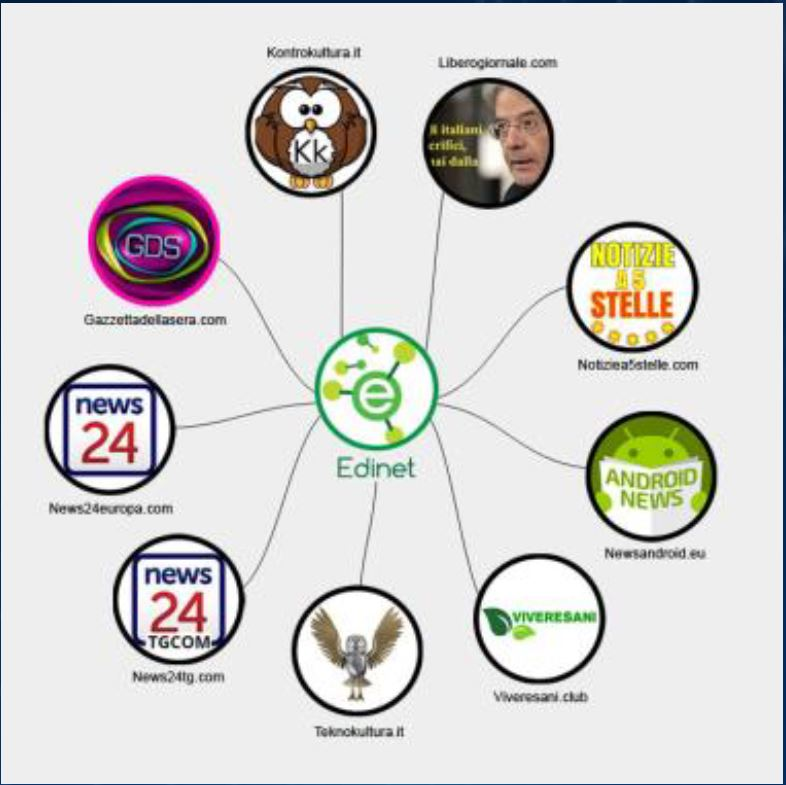
\includegraphics[width=0.5\textwidth]{images/10_lez_fig_01.jpg}
\end{figure}


Anche attraverso questo sistema è possibile moltiplicare la diffusione dell'informazione che viene diffusa. 

\subsection{Analfabetismo}
Un altro tema importante che gioca un ruolo fondamentale è l'analfabetismo. Parliamo di analfabetismo funzionale e di analfabetismo digitale. 
L'analfabetismo digitale normalmente caratterizza persone di una generazione non nata nel mondo digitale. Spesso le persone nate con le informazioni tradizionali non sanno gestire in modo completo e corretto lo strumento e si trovano in difficoltà quando si tratta di utilizzare gli strumenti che sono in continua evoluzione. 
Analfabetismo funzionale è quello che generalmente caratterizza i più giovani nativi digitali ma che non hanno acquisito una formazione sui contenuti e sulle possibilità di comprendere i contenuti tale da consettirgli di valutare l'attendibilità delle fonti e la correttezza delle informazioni.
Nell'autunno del 2016 l'Università di Stanford ha pubblicato uno studio dedicato proprio alla comprensione di come i giovani fra i 13-14 anni e 25 anni valutino la fonte delle informazioni e ne è emerso una grande incapacità di distinguere fra una fonte attendibile e una fonte inattendibile. 
Il ruolo nella diffusione sul web delle varie fonti è invece uguale. Non è detto che una fonte più attendibile o più seria abbia una capacità di diffusione delle informazioni maggiore di una fonte meno seria e meno attendibile. 
%20:05
\subsubsection{Facilità di pubblicazione}
Altro tema fondamentale pregio e difficoltà del web è la facilità con la quale si può arrivare a pubblicare qualsiasi tipo di commento. Qualunque utente sul web può generare contenuti informativi divulgandoli autoreferenziandosi. 
La grandissima differenza tra il web e i media tradizionali è proprio questa. Con i media tradizionali c'è un controllo, una verifica preliminare sull'informazione e soprattutto sull'autore dell'informazione per cui non tutto arriva a disposizione del pubblico. Basti pensare ad esempio ai giornali. Sui giornali scrivono i giornalisti professionisti, il pubblico può interagire, può commentare ma in un spazio ben preciso e ben dedicato che è quello delle lettere al giornale. 
Lo stesso discorso vale per la televisione. Il pubblico può interloquire, può partecipare come pubblico non come autore di nuovi contenuti. 
Nel web invece chiunque può aprire un blog, può pubblicare il proprio commento e può interagire con l'intero pubblico della rete.
Questo porta anche a delle conseguenze paradossali, ad esempio si trovano situazioni nelle quali il cittadino comune dibatte con l'esperto in una determinata materia pretendendo magari di spiegare come funzionano le cose. Qui mi piace citare una frase una dichiarazione di Piero Angela nel corso di un'intervista rilasciata nel febbraio-marzo del 2018 nella quale Piero Angela dice che la velocità della luce non si determina per alzata di mano. 
Occorre, nella possibilità di comunicare e dire la propria opinione,  trovare gli strumenti per distinguere fra un'opinione e una presa di posizione e un'affermazione di un esperto basata su ricerche, su fatti, su approfondimenti che non sono necessariamente del cittadino comune che si occupa magari di qualcos'altro. 

\subsubsection{Anonimato}
Altro tema importante è quello dell'anonimato. Sul web mediamente gli autori possono rimanere anonimi in primo luogo perché non c'è generalmente alcun obbligo né alcuna possibilità di controllo sulla effettiva identità di colui che apre un profilo, un account o che pubblica un commento. 
L'anonimato ha delle caratteristiche positive. Ci sono degli studi dell'UNESCO che chiariscono come la protezione dell'anonimato sia importante per le fonti giornalistiche in determinati contesti nei quali parlare liberamente è difficile. 
È anche vero che in alcune situazioni invece l'anonimato consente ai cosiddetti leoni da tastiera di diffondere informazioni di fare commenti, di denigrare il prossimo proprio con l'idea di non essere scoperti. 
Si dice anche che l'anonimato sul web è comunque una chimera perché spesso è possibile che la polizia postale, le autorità che fanno delle indagini, che hanno degli obblighi da adempiere rispetto a determinati contenuti che costituiscono un illecito possano rintracciare la persona.
Il fatto che sia possibile un anonimato porta anche ad una difficoltà di individuare se vi sono dei legami tra il sito informativo, tra l'informazione che viene distribuita e gruppi di potere. In altri termini, i legami fra un'informazione, fra i siti e determinati gruppi di potere può essere difficilmente riconoscibile con conseguente difficoltà quindi di comprendere quale sia l'effettiva fonte dell'informazione.
Ancora è possibile concentrare le fonti informative senza che questo sia immediatamente evidente. 
\subsubsection{Automazione}
\begin{itemize}
    \item I like e i profili sul web possono essere falsi. I profili possono essere creati da un unico soggetto o da più soggetti collegati ed essere replicati in maniera indiscriminata e incontrollabile. Anche i like su determinate immagini, notizie e post possono essere in realtà frutto di un'attività informatica di aumento di like con la conseguente ridistribuzione e ridiffusione sul web perché un contenuto che ha molti like viene indicizzato meglio, viene rivisto con più piacere perché anche l'utente che va a visualizzare le informazioni quando si rende conto che l'informazione ha un numero di visualizzazioni molto elevato, è invitato e aiutato ad andare ad aprire quell'informazione e a verificarla. In più, un numero di like molto importante contribuisce a creare una patente di attendibilità della notizia che viene diffusa.
    \item L'automazione consente anche un'aggregazione incontrollata e non trasparente fra informazioni diverse. È il fenomeno dell'indicizzazione delle informazioni che non è conosciuta né conoscibile da parte del grande pubblico.
    \item L'automazione consente una memoria locale delle ricerche precedentemente fatte. In altri termini, un utente che si pone davanti al web, quando cerca una determinata informazione, avrà facilmente restituite informazioni molto simili dello stesso tipo anche quando ritiene di fare una ricerca completamente nuova.
    \item L'automazione consente infatti di profilare le ricerche che sono state fatte dall'utente, consente di tenerne memoria e quindi in questo maniera consente di presentare all'utente che fa le sue ricerche delle informazioni molto simili, molto collegate, consente di restituirgli informazioni che il motore di ricerca o la piattaforma, o comunque il sistema, riconosce come informazioni che potrebbero essere gradite a chi fa la ricerca.



\end{itemize}

\subsubsection{Quali sono i rischi?}
\begin{itemize}
    \item un rischio è quello della manipolazione dell'informazione, quindi portare all'attenzione del pubblico un'informazione che è stata predigerita, precontrollata, premasticata in una maniera tale che un grande numero di persone continuerà ad essere convinta della verità di questa informazione.
    \item una delle preoccupazioni principali rispetto alla diffusione delle fake news è che queste possano essere un attentato ai processi politici e democratici. Nell'autunno del 2016, in occasione delle elezioni del presidente Trump negli Stati Uniti, si è cominciato a parlare dei rischi e della possibilità che le elezioni fossero state in qualche modo pilotate e controllate grazie alla diffusione di informazioni false sul web. All'epoca, autunno 2016, in inizio 2017, Facebook negò un suo possibile coinvolgimento, anche involontario, in un'operazione di questo tipo, è invece emerso nei primi mesi del 2018 che la società Cambridge Analytica avrebbe consentito avrebbe consentito la creazione di profili falsi su Facebook, i quali, a quanto sembrerebbe, effettivamente hanno contribuito alla divulgazione di informazioni che avrebbero aiutato l'elezione del presidente Trump.
    \item  La preoccupazione è al momento enorme, tanto che l'allarme sociale è tale che negli ultimi mesi del 2017 sono state adottate una serie di iniziative in ambito internazionale e presso diversi paesi, iniziative sia di studio, sia  di carattere normativo, che manifestano come ci sia una grande preoccupazione.
\end{itemize}

\textit{C'è un breve filmato in cu si fa vedere che se informazini sono verificate ci sono molte meno reazioni, è un episodio legato ai mussulmani.}
La diffusione di una informazione senza verifica dei fatti porta a una diffusione maggiore dell'odio. 
\begin{figure}[h]
    \centering
    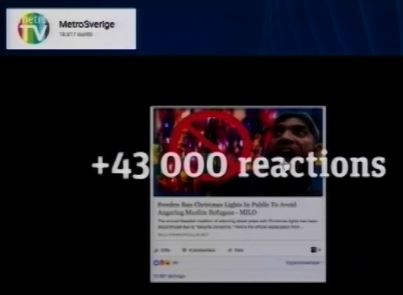
\includegraphics[width=0.5\textwidth]{images/10_lez_fig_02}
\end{figure}
Questo è realmente accaduto. Fact checking e non fact checking. 

\subsubsection{le dimensioni del fenomeno delle fake news}
Altro tema importante sono le dimensioni del fenomeno. Il fenomeno delle fake news ha due diverse dimensioni.
C'è un aspetto pubblico. L'interesse collettivo ad avere un'informazione corretta. La collettività nel suo insieme ha interesse a un'informazione corretta. Questo interesse della collettività si contrappone in qualche modo o comunque è un'altra faccia della medaglia dell'informazione perché dall'altro lato nelle società occidentali ognuno ha diritto di esprimersi liberamente e quindi di dire la propria versione. 
Per cui abbiamo un primo tema che è quello dell'interesse a informare da un lato dell'interesse a essere informati dall'altro. Nell'interesse a essere informati c'è l'importanza di un'informazione corretta. 
La pubblicazione di una notizia, di un'informazione può avere come contraltare quello di andare a toccare gli interessi di una singola persona. Quindi la seconda dimensione dell'informazione e della diffusione dell'informazione è l'interesse privato del singolo alla tutela della propria reputazione, alla tutela della propria identità, al diritto all'oblio di cui molto si parla e di cui avremo l'occasione di parlare meglio in una delle prossime lezioni. 
Il diritto pubblico ad avere determinate informazioni può essere in contrasto con l'interesse del singolo a veder cancellate quelle informazioni. La valutazione sul compromesso da adottare sulla prevalenza dell'uno o dell'altro è una valutazione che dovrà essere fatta caso per caso. 

\subsubsection{quali sono i possibili rimedi?}
Quali sono i possibili rimedi rispetto alla diffusione delle fake news? Ci sono tre orientamenti nel mondo occidentale su quali siano gli strumenti di contrasto rispetto alla diffusione delle fake news.
\begin{itemize}
    \item Un primo rimedio che lascia al lettore la valutazione è un approccio sostanzialmente liberista si dice è il lettore che deve essere formato e informato e migliorando le proprie competenze sarà in grado di individuare, di selezionare le informazioni corrette da quelle non corrette quindi è importante che sia il lettore a farsi una propria idea. 
    \item Un secondo orientamento propone che siano i fornitori di servizi internet a fare un'attività di verifica sulle notizie diffuse e di eventuale eliminazione delle notizie false. Sulla scorta di questo tipo di impostazione nel dicembre del 2017 Facebook ha proposto l'introduzione di un pulsante antibufala. Si tratterebbe di una sorta di bottone rosso che consente al pubblico, agli utenti di segnalare se un contenuto che è stato pubblicato è un contenuto discutibile, non reale.Dopodiché nel momento in cui c'è un gran numero di segnalazioni Facebook dovrebbe fare una verifica con dei fact checkers, cioè con delle organizzazioni riconosciute, accreditate di verifica dei fatti e poi eliminare l'informazione se è falsa o comunque segnalare che si tratta di un'informazione falsa. Questo tipo di soluzione presenta delle difficoltà perché si lascia sostanzialmente nelle mani di soggetti privati, di multinazionali che hanno come principale obiettivo il profitto, la valutazione su ciò che è vero e ciò che non è vero.
    \item La terza possibilità di intervento prevede l'intervento dei governi. I singoli governi o meglio ancora gli organismi internazionali dovrebbero prevedere un obbligo di verifica, segnalazione e rimozione con una valutazione però fatta da organismi di carattere internazionale e con la previsione di sanzioni a carico di coloro che pubblicano le fake news o che le lasciano in linea nel momento in cui sanno che si tratta di notizie false. Rispetto a questo tipo di soluzione le perplessità sono legate alla paura che da questo possa derivarne una forma di censura rispetto all'informazione pubblicata. 
\end{itemize} 

Non c'è quindi una presa di posizioni unica su quale sia il modo di risolvere le questioni.

Semplice domanda: perché le fake news diffuse sul web sono diverse da quelle diffuse sui media tradizionali? Cosa sono le fake news? 





